\chapter{Proposta}
\label{ch:proposta}

A proposta principal deste trabalho é desenvolver uma versão do algoritmo FSS aplicando em problemas dinâmicos com domínio contínuo. Será aplicado as técnicas de manutenção da diversidade populacional estudadas neste trabalho, para avaliar a influência de cada uma em cada aspécto do algortimo, como performance, robustês e satisfabilidade. O algoritmo final terá a possibilidade de alternar nos operadores evolutivos, de modo que cada operador possa ser analisado individualmente (aplicado no FSS) ou em conjunto com outro operador e/ou técnica de manutenção de diversidade populacional.

Com este algoritmo será possível realizar experimentos para validar a relevância dos operadores utilizados para cada classe de problemas, como problemas com dinâmismos na função objetivo, no limite das variáveis ou até problemas com restrições dinâmicas. Além disso será possível analisar a interação dos operadores entre si e entre as técnicas de manutenção da diversidade populacional.

Para a realização dos testes serão aplicadas as mesmas métricas de performance, satisfabilidade, robustez e diversidade para realizar uma comparação justa e detalhada dos componentes usados no algoritmo final. Com o íntuito de melhor entender os componentes e o comportamento do algoritmo FSS, este foi implementado na sua versão canônica estacionária e um estudo de caso é detalhado a seguir na Seção \ref{sec:test_case}.

\section{Estudo de Caso}
\label{sec:test_case}

O algoritmo foi aplicado nas seguintes funções de \textit{benchmarks} estáticos: Rosembrock, Rastrigin, Griewank, Ackley e Schefel 1.2 que são descritas a seguir.

\begin{equation}
\label{eq:rosembrock}
F_{Rosembrock}(x) = \sum_{i=1}^{n-1} \left[ 100 (x_{i+1} - x_i^2)^2 + (1 - x_i)^2\right]
\end{equation}

\begin{figure}[!htb]
	\caption{Representação gráfica da função de Rosembrock}
	\centering
	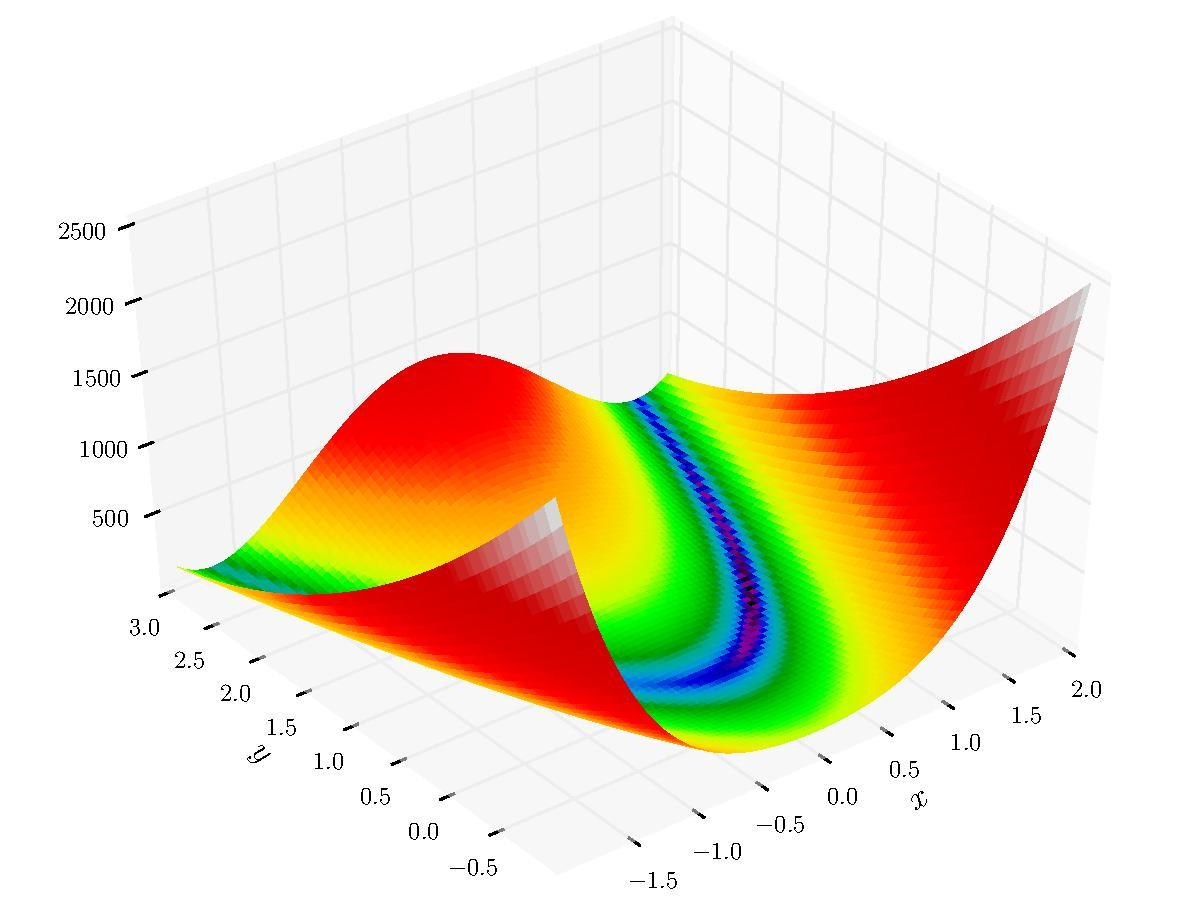
\includegraphics[scale=0.3]{images/f_rosembrock.jpg}
	\label{fig:f_rosembrock}
\end{figure}

\begin{equation}
\label{eq:rastrigin}
F_{Rastrigin}(x) = 10 n + \sum_{i=1}^{n} \left[ x_i^2 - 10\cos(2\pi x_i)\right]
\end{equation}

\begin{figure}[!htb]
	\caption{Representação gráfica da função de Rastrigin}
	\centering
	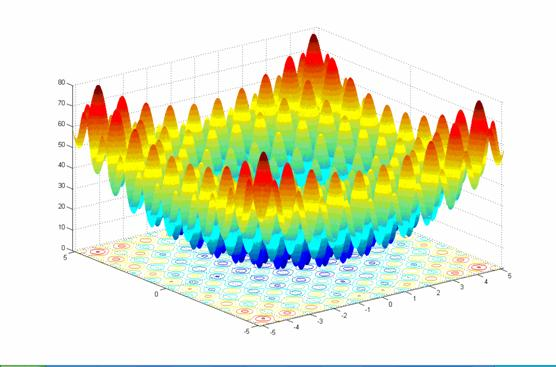
\includegraphics[scale=0.5]{images/f_rastrigin.jpg}
	\label{fig:f_rastrigin}
\end{figure}

\begin{equation}
\label{eq:griewank}
F_{Griewank}(x) = 1+ \sum_{i=1}^{n} \frac{x_i^2}{4000} - \prod_{i=1}^{n} \cos \left(\frac{x_i}{\sqrt{i}}\right)
\end{equation}

\begin{figure}[!htb]
	\caption{Representação gráfica da função de Griewank}
	\centering
	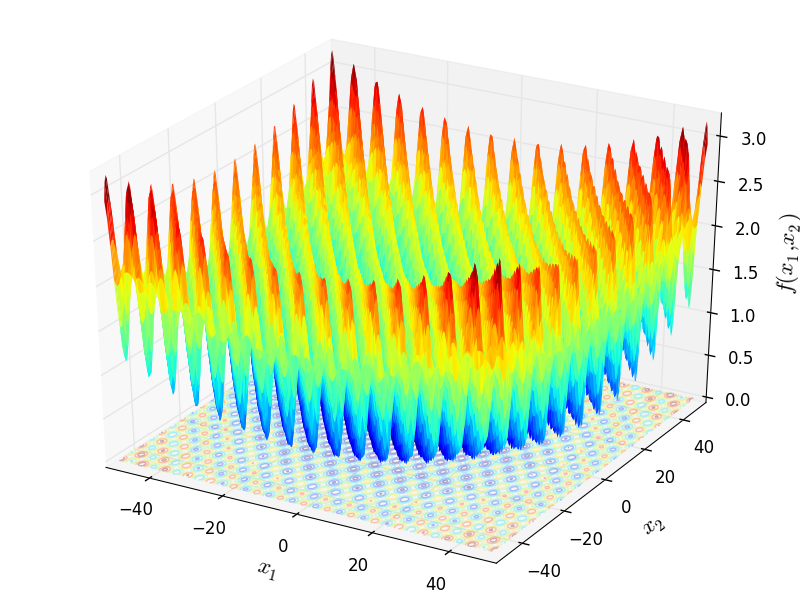
\includegraphics[scale=0.3]{images/f_griewank.png}
	\label{fig:f_griewank}
\end{figure}

\begin{equation}
\label{eq:ackley}
F_{Ackley}(x) = -20 \exp \left(-0.2 \sqrt{\frac{1}{n} \sum_{i=0}^{n} x_i^2 }\right) - \exp \left(\frac{1}{n} \sum_{i=0}^{n} \cos(2 \pi x_i) \right) + 20 + e
\end{equation}

\begin{figure}[!htb]
	\caption{Representação gráfica da função de Ackley}
	\centering
	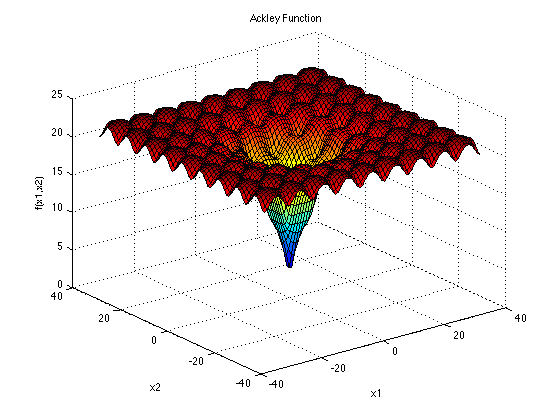
\includegraphics[scale=0.3]{images/f_ackley.png}
	\label{fig:f_ackley}
\end{figure}

\begin{equation}
\label{eq:schafel_12}
F_{Schefel 1.2}(x) = \sum_{i=0}^{n} \left(\sum_{j=0}^{i} x_i\right)^2
\end{equation}

\begin{figure}[!htb]
	\caption{Representação gráfica da função de Schafel}
	\centering
	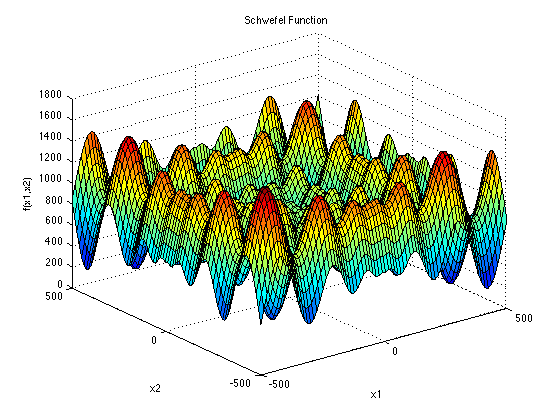
\includegraphics[scale=0.3]{images/f_schafel.png}
	\label{fig:f_schafel}
\end{figure}

Nos testes foram feitas 10 aplicações para cada função, utilizando: 30 dimensões, 30 peixes e 5.000 iterações sendo que o o número total de avaliações de \textit{fitness} é de 300.000. O parâmetros do FSS foram: o $step_{ind}$ inicial de 0,01 e o final de 0,00001, o $step_{vol}$ inicial de 0,01 e final de 0,0001 e o peso inicial de 2500, variando de 1 a 5000.
	Os Resultados obtidos estão apresentados na Tabela \ref{tb:results}
	
\begin{table}[]
	\centering
	\caption{Tabela de resultados do FSS canônico}
	\label{tb:results}
	\begin{tabular}{|c|c|c|}
		\hline
		\multicolumn{1}{|l|}{Problemas} & \multicolumn{1}{l|}{Melhor Resultado} & \multicolumn{1}{l|}{Desvio Padrão} \\ \hline
		Rosembrock                      &                                       &                                    \\ \hline
		Rastrigin                       &                                       &                                    \\ \hline
		Griewank                        &                                       &                                    \\ \hline
		Ackley                          &                                       &                                    \\ \hline
		Schafel 1,2                     &                                       &                                    \\ \hline
	\end{tabular}
\end{table}